\section{Mathematical Foundations}
This section serves as a short introduction to the mathematical concepts used throughout this paper. The reader should be familiar with the most basic concepts of probability theory and measure theory, such as probability spaces, sigma algebras, filtrations and measures.

This section is organized as follows. First, the above description of a real world problem is translated into the context and notation of probability theory. Then the resulting abstract mathematical description is transformed into a numerically tangible formulation.
\subsection{Notation}
We will only deal with stochastic processes with discrete time steps. These time steps will be indexed from 1 to a final time T. For a stochastic process $\xi$ with a continuous distribution, $\xi^t$ denotes the mapping from events to outcomes at time step $t$. For discrete stochastic processes, index sets for the events, typically denoted by $I$ and $J$, are introduced. For convenience, the stochastic process and its index set are used interchangeably. The outcome of an event $i\in I$ of a discrete stochastic process $\xi$ at time step $t$ is denoted by $\xi_i^t$. If the time step is omitted, this denotes the full scenario $i$, that is the vector of the values $\xi_i^t$ sorted by their times $t$.

The vector $e$ denotes a vector of ones in each dimension. The dimension will be chosen in accordance with the context. 

In optimization problems, if there are indices in an equation that are not explicitly declared, it is assumed that this equation is stated for each of the indices in the corresponding set.
The corresponding set will always be obvious in context.

For a set $A$, $\mathfrak{P}(A)$ denotes the power set.
\subsection{Stochastic Programming and Scenario Trees}
Suppose a problem given in the following generic nonlinear multi-stage stochastic structure. 
\begin{eqnarray}
  \label{eq:genericSP}
  \min &&\mathbb{E}\left[\sum_{t=1}^Tf_t(\xi_t, x_t)\right]\\
  &\mathrm{s.t.}& h_t(\xi_t, x_t, x_{t-1}) = 0\\
  &&x_t \in X_t\\
  &&x_t \, \mathrm{is}\,\mathcal{F}_t \mathrm{-measurable} \label{eqn:measurability-constraint}
\end{eqnarray}
In this problem, the stochastic process $\xi$ can be considered as a mapping $\xi:\Omega\rightarrow \mathbb{R}^{d\times T}$, where $\Omega$ is the sample space of the underlying probability space $(\Omega, \mathcal{F}, \mathbb{P})$. The solution is a mapping $x:\Omega\rightarrow \mathbb{R}^{n\times T}$.

The difficulty in multi-stage stochastic programming problems arises from the measurability constraint (\ref{eqn:measurability-constraint}). This constraint is specific to multi-stage stochastic programs.
This additional constraint leads to a much increased computational complexity of multi-stage programs over two-stage programs \cite{Shapiro2005,Shapiro2008}.
% 
\par{Measurability Constraints} 
mean that the condition
\begin{equation}
  \label{eq:mathematical-NAC}
  \omega_1,\omega_2\in \Omega \, : \, \xi_\tau(\omega_1) = \xi_\tau(\omega_2)\,\forall \tau\leq t\,\Rightarrow \, x_t(\omega_1) = x_t(\omega_2) 
\end{equation}
has to hold for all time steps $t$, and all pairs of events $(\omega_1,\omega_2)$. 
Note that this implies that the decision variables $x_t$ must only depend on the events of the past up until the present $\xi_1$, ..., $\xi_t$, and explicitly \textbf{not} on $\xi_{t+1},\, ...,\,\xi_T$. 
This property is often called \textit{non-anticipativity of the solution} $x$. 
Therefore, these equations model the uncertainty of the future.
% 
\paragraph{Discretization}
% 
Stochastic Programs are infinite dimensional optimization problems and as such not immediately accessible to computation.
To transform the stochastic program into a computable problem, the infinite dimensional stochastic process $\xi$ must be discretized into a finite stochastic process $\hat{\xi}$ (see figure \ref{fig:abstract-discretization}). 
\pgfdeclarelayer{background}
\pgfsetlayers{background,main}
\begin{figure}
  \centering
    \begin{tikzpicture}[node distance=5cm, auto]
      \node [block] (xiorig) {$\xi$};
      \node [block, below of=xiorig] (xi) {$\hat{\xi}$};
      \node [block, text width=10em, right of=xiorig] (infsolver){Infinite Dim. Solver};
      \node [block, right of=infsolver] (xorig){$x$};
      \node [block, text width=10em, below of=infsolver] (nlp) {(N)LP Solver};
      \node [block, below of=xorig] (x) {$x$};

      \path [line] (xiorig) -- node (xierror) {$D(\xi,\hat{\xi})$} (xi);
      \path [line] (x) -- node (xerror) {$D(x,\hat{x})$} (xorig);
      \path [line,dashed] (xierror) -- node {$L\cdot D(\xi,\hat{\xi})\geq D(x,\hat{x})$} (xerror);
      \path [line] (xiorig) -- (infsolver);
      \path [line] (xi) -- (nlp);
      \path [line] (nlp) -- (x);
      \path [line] (infsolver) -- (xorig);

      \node [node distance=1.4cm,below of=xi] (focus){Focus of this paper};
      \begin{pgfonlayer}{background}
        \node (selection) [draw, rounded corners,dotted, fill=orange!20, fit=(xiorig) (xi) (xierror) (focus)] {};
      \end{pgfonlayer}
    \end{tikzpicture}
  \caption{Steps in the discretization of a stochastic program. Since the infinite dimensional solver is just a theoretical enitiy, The path below must be used. A discretization error is introduced when converting $\xi$ to $\hat{\xi}$. This error is propagated through the NLP. For linear stochastic programs, \cite{Heitsch2010} have shown that there exists a problem specific constant $L$ such that the error between the discretized and the original solution is bounded by the error in the discretization of the stochastic process.}
  \label{fig:abstract-discretization}
\end{figure}
If certain precautions are taken, it is possible to show (at least for linear stochastic programs) that the solution to the stochastic problem is stable under this discretization operation, meaning that there exists a factor $L$ such that the distance between the solution to the discretized problem $\hat{x}$ and the solution to the original problem $x$ are Lipschitz-continuous with respect to the discretization error:
\begin{equation}
  D(x , \hat{x}) \leq L\cdot D(\xi,\hat{\xi})
\end{equation}
where $D$ is an appropriate norm. See \cite{Heitsch2010} for the proof and further details. The correct choice for $D$ will be discussed in sections \ref{sec:measuring-challenges} and \ref{sec:kantoro}.

The discretization will be carried out in two steps. 
First, the infinite dimensional stochastic process $\xi$ is approximated by a set of scenarios sampled using Monte-Carlo techniques. 
This step is well known and will not be discussed here. 
To capture the essence of the non-anticipativity constraints, in a second step the scenarios $I$ are recombined into a tree structure. 

Tree structures introduce the non-anticipativity constraints in intuitive way (see figure \ref{fig:violated-nonanticipativity}.
The parent node holds the information of the past, while each node is branched into multiple possible future states. 
It is, in fact, insufficient to represent the stochastic process as a set of non-interdependent scenarios with a common root. 
As this is a common misconception, for illustration purposes we will give the following
\begin{example}[Necessity of tree structure]
  \label{ex:tree-necessity}
  % \hangindent=1cm
  Consider a game of coin tosses, played by a player against a bank. 
  The player will play the game for three consecutive coin tosses. 
  He has three Euros that he all wants to bet. 
  Predicting the outcome of the toss correctly will return 
  \begin{itemize}
  \item $\frac{13}{6}$ the stakes $x$ in the first round,
  \item $2\cdot x$ in the second round,
  \item and only $1.5\cdot x$ in the final round.
  \end{itemize}
  Otherwise the stakes will be lost. 
  Earnings cannot be used to bet in the game.

  The player optimizes the expected return.
  Without the need for a calculator we can say that the optimal strategy is to bet everything in the first round, yielding a total expected return of $1.75$.

  Consider now a transcription of the problem as an LP, using all possible scenarios (see figure \ref{fig:violated-nonanticipativity}, top).
  For three consecutive coin tosses, there are eight different scenarios.
  The player wants to use this LP to help him decide, how much he is supposed to bet in the first round.
  The corresponding LP is
  \begin{align*}
    \min\limits_x &\; \sum_{s\in S}\sum_{t=1}^3p_sx_s^t\cdot c_s^t\\
    \text{s.t.} &\; \sum_{t=1}^3x_s^t = 3 \;\forall\, s\in S\\
    & \; x_s^1 = x_0^1\;\forall s\in S
  \end{align*}
  where $S$ is the set of scenarios, $c_s^t$ is the outcome of the game (return per Euro for win, $0$ for loss), $x_s^t$ is the amount that the player is willing to bet at time step $t$ in scenario $s$. The first equation ensures that the player spends exactly the amount he has at his disposal. The second equation fixes the players decision in the first round.

  The results, summarized in table \ref{tab:coin-toss-results}, show that the solution of the LP does not match the optimal solution, even though the uncertainty was seemingly taken into account. 
  The flaw in the above formulation is that the non-anticipativity constraints are missing for stage 2. 
  The algorithm believes to know what will happen, as soon as the first value is revealed. 
  The game, as it is modeled in the LP is as follows: 
  ``Make one decision with stochastic outcome, then make two decisions with perfect foresight''. 
  In this situation, the algorithm will correctly decide to wait and spend its money only on bets that it knows the result of beforehand (see figure \ref{fig:violated-nonanticipativity}). 
  \begin{figure}
  \centering
    \begin{tikzpicture}
      \node (root) at (0,0) [circle,draw] {$x_{\mathrm{now}}$};
      \node (n11) at (2,3.5) [circle,draw]  {W};
      \node (n12) at (2,2.5) [circle,draw]  {W};
      \node (n13) at (2,1.5) [circle,draw]  {W};
      \node (n14) at (2,0.5) [circle,draw]  {W};
      \node (n18) at (2,-3.5) [circle,draw] {L};
      \node (n17) at (2,-2.5) [circle,draw] {L};
      \node (n16) at (2,-1.5) [circle,draw] {L};
      \node (n15) at (2,-0.5) [circle,draw] {L};

      \node (n21) at (4,3.5) [circle,draw]  {$x_{11}$};
      \node (n22) at (4,2.5) [circle,draw]  {$x_{12}$};
      \node (n23) at (4,1.5) [circle,draw]  {$x_{13}$};
      \node (n24) at (4,0.5) [circle,draw]  {$x_{14}$};
      \node (n28) at (4,-3.5) [circle,draw] {$x_{18}$};
      \node (n27) at (4,-2.5) [circle,draw] {$x_{17}$};
      \node (n26) at (4,-1.5) [circle,draw] {$x_{16}$};
      \node (n25) at (4,-0.5) [circle,draw] {$x_{15}$};

      \node (n31) at (6,3.5) [circle,draw]  {W};
      \node (n32) at (6,2.5) [circle,draw]  {W};
      \node (n33) at (6,1.5) [circle,draw]  {L};
      \node (n34) at (6,0.5) [circle,draw]  {L};
      \node (n38) at (6,-3.5) [circle,draw] {L};
      \node (n37) at (6,-2.5) [circle,draw] {L};
      \node (n36) at (6,-1.5) [circle,draw] {W};
      \node (n35) at (6,-0.5) [circle,draw] {W};

      \node (n41) at (8,3.5) [circle,draw]  {$x_{21}$};
      \node (n42) at (8,2.5) [circle,draw]  {$x_{22}$};
      \node (n43) at (8,1.5) [circle,draw]  {$x_{23}$};
      \node (n44) at (8,0.5) [circle,draw]  {$x_{24}$};
      \node (n48) at (8,-3.5) [circle,draw] {$x_{28}$};
      \node (n47) at (8,-2.5) [circle,draw] {$x_{27}$};
      \node (n46) at (8,-1.5) [circle,draw] {$x_{26}$};
      \node (n45) at (8,-0.5) [circle,draw] {$x_{25}$};

      \node (n51) at (10,3.5) [circle,draw]  {W};
      \node (n52) at (10,2.5) [circle,draw]  {L};
      \node (n53) at (10,1.5) [circle,draw]  {W};
      \node (n54) at (10,0.5) [circle,draw]  {L};
      \node (n58) at (10,-3.5) [circle,draw] {L};
      \node (n57) at (10,-2.5) [circle,draw] {W};
      \node (n56) at (10,-1.5) [circle,draw] {L};
      \node (n55) at (10,-0.5) [circle,draw] {W};

      \draw (root) -- (n11);
      \draw (root) -- (n12);
      \draw (root) -- (n13);
      \draw (root) -- (n14);
      \draw (root) -- (n15);
      \draw (root) -- (n16);
      \draw (root) -- (n17);
      \draw (root) -- (n18);

      \draw (n11) -- (n21);
      \draw (n12) -- (n22);
      \draw (n13) -- (n23);
      \draw (n14) -- (n24);
      \draw (n15) -- (n25);
      \draw (n16) -- (n26);
      \draw (n17) -- (n27);
      \draw (n18) -- (n28);

      \draw (n21) -- (n31);
      \draw (n22) -- (n32);
      \draw (n23) -- (n33);
      \draw (n24) -- (n34);
      \draw (n25) -- (n35);
      \draw (n26) -- (n36);
      \draw (n27) -- (n37);
      \draw (n28) -- (n38);

      \draw (n31) -- (n41);
      \draw (n32) -- (n42);
      \draw (n33) -- (n43);
      \draw (n34) -- (n44);
      \draw (n35) -- (n45);
      \draw (n36) -- (n46);
      \draw (n37) -- (n47);
      \draw (n38) -- (n48);

      \draw (n41) -- (n51);
      \draw (n42) -- (n52);
      \draw (n43) -- (n53);
      \draw (n44) -- (n54);
      \draw (n45) -- (n55);
      \draw (n46) -- (n56);
      \draw (n47) -- (n57);
      \draw (n48) -- (n58);

    \begin{pgfonlayer}{background}
        \node [fit=(n11) (n24), fill=orange!20] {};
      \end{pgfonlayer}
\end{tikzpicture}
    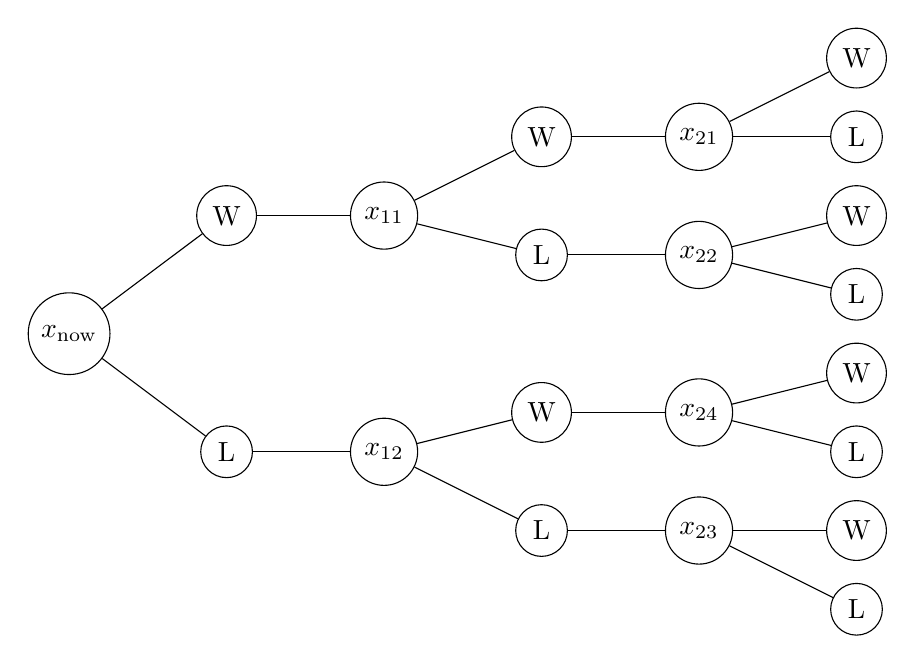
\begin{tikzpicture}
      \node (root) at (0,0) [circle,draw] {$x_{\mathrm{now}}$};

      \node (n1) at (2,1.5) [circle, draw] {W};
      \node (n2) at (2,-1.5) [circle, draw] {L};

      \draw (root) -- (n1);
      \draw (root) -- (n2);
      
      \node (n3) at (4,1.5) [circle, draw] {$x_{11}$};
      \node (n4) at (4,-1.5) [circle, draw] {$x_{12}$};

      \draw (n1) -- (n3);
      \draw (n2) -- (n4);

      \node (n5) at (6,2.5) [circle, draw] {W};
      \node (n6) at (6,1) [circle, draw] {L};
      \node (n7) at (6,-2.5) [circle, draw] {L};
      \node (n8) at (6,-1) [circle, draw] {W};

      \draw (n3) -- (n5);
      \draw (n3) -- (n6);
      \draw (n4) -- (n7);
      \draw (n4) -- (n8);
      
      \node (n9) at (8,2.5) [circle, draw] {$x_{21}$};
      \node (n10) at (8,1) [circle, draw] {$x_{22}$};
      \node (n11) at (8,-2.5) [circle, draw] {$x_{23}$};
      \node (n12) at (8,-1) [circle, draw] {$x_{24}$};

      \draw (n5) -- (n9) ;
      \draw (n6) -- (n10);
      \draw (n7) -- (n11);
      \draw (n8) -- (n12);

      \node (n13) at (10,3.5) [circle,draw]  {W};
      \node (n14) at (10,2.5) [circle,draw]  {L};
      \node (n15) at (10,1.5) [circle,draw]  {W};
      \node (n16) at (10,0.5) [circle,draw]  {L};
      \node (n17) at (10,-3.5) [circle,draw] {L};
      \node (n18) at (10,-2.5) [circle,draw] {W};
      \node (n19) at (10,-1.5) [circle,draw] {L};
      \node (n20) at (10,-0.5) [circle,draw] {W};

      \draw (n9) -- (n13);
      \draw (n9) -- (n14);
      \draw (n10) -- (n15);
      \draw (n10) -- (n16);
      \draw (n11) -- (n17);
      \draw (n11) -- (n18);
      \draw (n12) -- (n19);
      \draw (n12) -- (n20);
      
    \end{tikzpicture}
    \caption{The non-anticipativity constraints are violated in the first plot. Variables $x_{11},\ldots x_{14}$ share the identical history $\xi_{11}=\ldots = \xi_{14}=W$. Therefore, they must be identical. The tree structure below solves this problem by only introducing one variable for each distinct history.}
  \label{fig:violated-nonanticipativity}
\end{figure}
  \begin{table}
    \small\centering
    \begin{tabular}{lcccccccc}
      \hline 
      Scenario&1&2&3&4&5&6&7&8\\\hline\hline
      Result&WWW&WWL&WLW&WLL&LWW&LWL&LLW&LLL\\
      Opt. Solution&300&300&300&300&300&300&300&300\\
      LP Solution&030&030&003&003&030&030&003&003\\\hline
    \end{tabular}
    \vspace*{0.5cm}\\
    \begin{tabular}{lcc}
      \hline
      &Opt. Solution&LP Solution\\\hline\hline
      Opt. Value (computed)&1.75&1.875\\
      Opt. Value (real)&1.75&1.5\\
      \hline
    \end{tabular}
    \caption{Results of the coin-toss example}
    \label{tab:coin-toss-results}
  \end{table}
\end{example}

The above example illustrates the need for tree structured stochastic processes. The construction of this tree structure will be the main point of the following paper. Before we can start constructing these scenario trees, we need to define a measure for the quality of a given approximation $\hat{\xi}$ to a stochastic process $\xi$. The goal is to define a distance function 
\begin{equation}
  \label{eq:distance-function-intro}
  D:\mathcal{S} \times \mathcal{S} \rightarrow \mathbb{R}_+,\;(\xi, \hat{\xi})\mapsto D(\xi, \hat{\xi})
\end{equation}
where $\mathcal{S}$ is the space of stochastic processes which remains to be defined. The distance function should satisfy at least the definition of a metric. Since the choices for $\mathcal{S}$ and $D$ are by no means obvious, they are discussed in the following section.
\subsection{Challenges in Measuring Stochastic Processes}
\label{sec:measuring-challenges}
The purpose of this section is to derive a distance function (\ref{eq:distance-function-intro}) which will serve as a means to evaluate the quality of a scenario tree approximation to a stochastic process.
As we are dealing mainly with the numerics of this problem, the theoretical discussion is carried out with a focus on comprehensibility.
For a detailed and mathematically thorough discussion see \cite{Heitsch2010} and the references therein.

Stochastic processes are very versatile and complex objects.
Depending on the problem at hand, different interpretations may be useful. 

In general, a stochastic process (as stated above, we will focus exclusively on time-discrete stochastic processes) is a composition of five objects. The first three objects compose a probability space: a sample space $\Omega$, a filtration (family of $\sigma$-algebras) $\left\{\mathcal{F}_t\right\}_{t=1}^T$, and a probability measure $\mathbb{P}$ which is a mapping from the set of distinguishable events at time $t$ to a probability:
\begin{equation}
  \label{eq:prob-measure-definition}
  \mathbb{P}_t : \mathcal{F}_t \rightarrow \left[0,1\right]. 
\end{equation}
The final two elements of the stochastic process are a set of values that the stochastic process can take, and a mapping $\zeta$ from the sample space to the value space. For our purposes, the value space will always be a subset of the Euclidean space $\mathbb{R}^n$.

These elements that make up the stochastic process can lead to different interpretations, by fixing four of these five and considering the space of stochastic processes in terms of the fifth object. One popular way to do this is to fix everything but the mapping $\zeta$ from the sample space to the value space. An example of this usage is the proof of the stability properties of multi-stage stochastic linear programs in (\cite{Heitsch2010}). The corresponding space is the space of functions mapping $\Omega$ to $\mathbb{R}^n$. The exact space depends on the regularity of the functions one would like to consider. A natural choice is the space of p-integrable functions $L^p$ since there is no reason for the assumption of any kind of differentiability of $\zeta$ and $L^p$ has the nice feature of being a Banach Space, which allows for the definition of a norm
\begin{equation}
  \label{eq:Lp-norm}
  \left\Vert\xi\right\Vert_p = \sum_{t=1}^T\left(\int_{\omega\in \Omega}\left\Vert\zeta_t(\omega)\right\Vert^p d\mathbb{P}(\omega)\right)^{1/p}.
\end{equation}

The most common way to think about stochastic processes is, however, in terms of its probability measure $\mathbb{P}$.
For the purpose of this discussion, let $\Omega=\mathbb{R}^n$ and $\zeta=id$.
Each of the elements of the stochastic process except for the probability measure is fixed, and the stochastic process is considered in terms of the space of probability measures.
This interpretation will be followed throughout this paper.

The choice of the space of probability measures as the underlying space for stochastic processes leads to much more difficulties when defining a metric. It is not feasible to regard two probability measures $\mathbb{P}_1$ and $\mathbb{P}_2$ as integrable functions and elements of $L^p$ for two reasons:
\begin{enumerate}
\item The metric between two stochastic processes $\xi_1$ and $\xi_2$ would be defined in terms of the $L^p$-norm between their probability measures $\mathbb{P}_1$ and $\mathbb{P}_2$:
  \begin{equation}
    \label{eq:prob-measure-metric-as-Lpnorm}
    D(\mathbb{P}_1,\mathbb{P}_2) := \left\Vert \mathbb{P}_1-\mathbb{P}_2\right\Vert = \sum_{t=1}^T\int_{\omega\in\Omega}\left\Vert \mathbb{P}_{1,t}(\omega)-\mathbb{P}_{2,t}(\omega)\right\Vert
  \end{equation}
  This does, however, not yield meaningful results. See figure \ref{fig:example-wrong-distance} for an example.
\item The definition of the above metric makes use of the pointwise difference of $\mathbb{P}_1$ and $\mathbb{P}_2$
  This difference is, however, not a meaningful construction, since the difference of two probability measure functions is itself \textbf{never} a probability measure.
\end{enumerate}
\begin{figure}
  \centering
  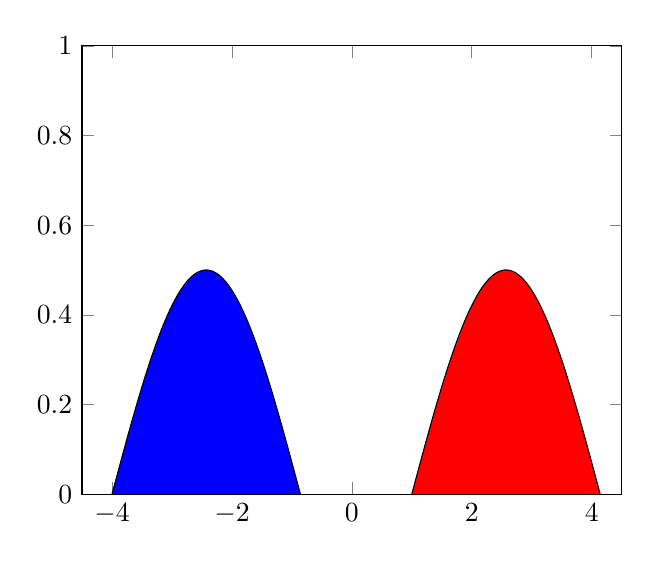
\begin{tikzpicture}
    \begin{axis}[ymin=0, ymax=1, xmin=-4.5, xmax=4.5]
      \addplot[domain=-4:-0.8584,samples=100,fill=blue]{sin(deg(x+4))/2};
      \addplot[domain=1:4.1416,samples=100, fill=red]{sin(deg(x-1))/2};
      \end{axis}
  \end{tikzpicture}
  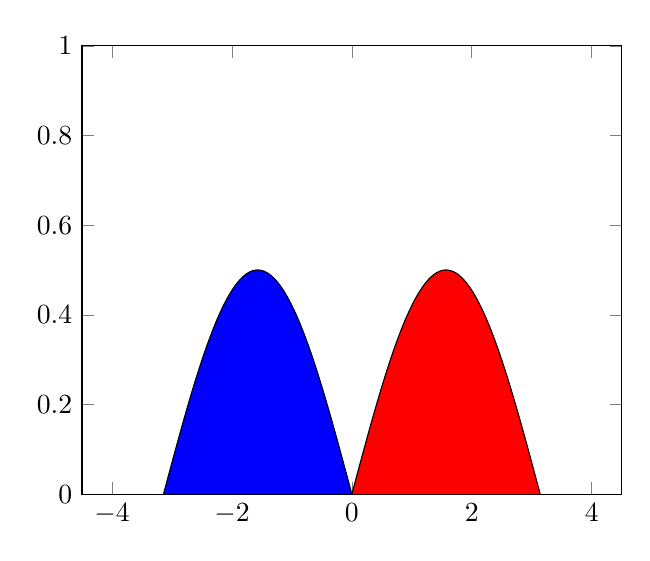
\begin{tikzpicture}
    \begin{axis}[ymin=0, ymax=1, xmin=-4.5, xmax=4.5]
      \addplot[domain=-3.1416:0,samples=100,fill=blue]{sin(deg(x+3.1416))/2};
      \addplot[domain=0:3.1416,samples=100, fill=red]{sin(deg(x))/2};
    \end{axis}
  \end{tikzpicture}
  % \missingfigure{two probability distributions moving closer together but same distance}
  \caption{Example of two different probability distances. 
    Even though the probability distributions of the second plot are closer than the ones on the first plot, they have the same distance in the $L^p$ norm.}
  \label{fig:example-wrong-distance}
\end{figure}

\subsection{The Kantorovich Distance}
\label{sec:kantoro}
In this section, we will present the Kantorovich Distance as a meaningful and usable metric for stochastic processes. For a gentle introduction to the Kantorovich Distance see \cite{Deng2009}.
% Note that stochastic processes can be represented as random variables by considering each trajectory as an event.

In the context of stability analysis of stochastic programming problems, it has been shown by \cite{Dupacova2003} that the Kantorovich functional
\begin{equation}
  \label{eq:define-infinitedim-kantorovich}
  \mu_c(\mathbb{P}, \mathbb{Q}) = \inf\left\{\int_{\Omega\times\Omega}c(\omega, \hat{\omega})\eta(d(\omega,\hat{\omega})),\, \eta\in\mathcal{M}\right\}
\end{equation}
represents a  ``natural and suitable''\cite{Dupacova2003} distance for measuring stochastic processes in the context of stochastic programming problems. 
Here, $\mathcal{M}(\mathbb{P, Q})$ is the space of Borel-measures with marginals $\mathbb{P}$ and $\mathbb{Q}$, meanging that $\eta$ is a probability measure on the space $\Omega\times\Omega$ with the properties
\begin{equation}
  \label{eq:define-borel-measures}
  \int_{B\times \Omega} \eta(d(\omega,\hat{\omega})) = \mathbb{P}(B),\;   \int_{\Omega\times B} \eta(d(\omega,\hat{\omega})) = \mathbb{Q}(B),\; B \in \mathcal{B}
\end{equation}
where $\mathcal{B}$ is the Borel-$\sigma$-field with respect to $\Omega$.
The distance $c$ is a mapping with certain properties, which are specified in \cite{Dupacova2003}.
For the purposes of this paper, it suffices to say that any vector norm satisfies these conditions.

\begin{Note}
  In this section, the Kantorovich Metric as applied to the stochastic process as a random variable has been proposed for measuring stochastic processes in stochastic programming.
  In the derivation of the stability of multistage stochastic processes (\cite{Heitsch2010}), the $L^p$ norm (\ref{eq:Lp-norm}) in conjunction with a ``filtration distance'' was used.
  Recently, it has been shown that previous heuristics (for example those in \cite{Dupacova2003}) that disregarded the filtration distance fail to uphold stability of the problem (\cite{Heitsch2009a}).
  These methods, as opposed to the one presented here, had obvious disregard for the filtration, because they were based on sums over all stages with stage-dependent terms.
  The methods for scenario tree construction presented in this paper ensure the correctness of the filtration through the tree structure, that is postulated beforehand.
\end{Note}
\paragraph{Kantorovich Distance for finite stochastic processes}
Besides its virtues for the stability analysis \cite{Dupacova2003}, an advantage of the Kantorovich Distance is its simple and intuitive representation for finite dimensional stochastic processes.
\begin{figure}
  \centering
  \begin{tikzpicture}
    \node [draw,ellipse, fill=red!20] (n1) at (0,0) {$p_1=0.1$};
    \node [draw,ellipse, fill=red!20] (n2) at (5.5,1) {$p_2=0.2$};
    \node [draw,ellipse, fill=red!20] (n3) at (10,7.5) {$p_3=0.1$};
    \node [draw,ellipse, fill=red!20] (n4) at (4.5,5.5) {$p_4=0.2$};
    \node [draw,ellipse, fill=red!20] (n5) at (12,1) {$p_5=0.1$};
    \node [draw,ellipse, fill=red!20] (n6) at (8,5) {$p_6=0.2$};
    \node [draw,ellipse, fill=red!20] (n7) at (0.5,8) {$p_7=0.1$};

    \node [draw,ellipse, fill=blue!20] (m1) at (2.3,3) {$q_1=0.3$};
    \node [draw,ellipse, fill=blue!20] (m2) at (5.5,7.5) {$q_2=0.4$};
    \node [draw,ellipse, fill=blue!20] (m3) at (9,3) {$q_3=0.3$};

    \path [line] (n1) -- node [rectangle, draw,fill=white] (eta11){$\eta_{11}=0.1$} (m1);
    \path [line] (n2) -- node [rectangle, draw,fill=white] (eta21){$\eta_{21}=0.1$} (m1);
    \path [line] (n2) -- node [rectangle, draw,fill=white] (eta23){$\eta_{23}=0.1$} (m3);
    \path [line] (n4) -- node [rectangle, draw,fill=white] (eta41){$\eta_{41}=0.1$} (m1);
    \path [line] (n4) -- node [rectangle, draw,fill=white] (eta42){$\eta_{42}=0.1$} (m2);
    \path [line] (n7) -- node [rectangle, draw,fill=white] (eta72){$\eta_{72}=0.1$} (m2);
    \path [line] (n3) -- node [rectangle, draw,fill=white] (eta32){$\eta_{32}=0.1$} (m2);
    \path [line] (n2) -- node [rectangle, draw,fill=white] (eta21){$\eta_{21}=0.1$} (m1);
    \path [line] (n5) -- node [rectangle, draw,fill=white] (eta53){$\eta_{53}=0.1$} (m3);
    \path [line] (n6) -- node [rectangle, draw,fill=white] (eta63){$\eta_{63}=0.1$} (m3);
    \path [line] (n6) -- node [rectangle, draw,fill=white] (eta62){$\eta_{62}=0.1$} (m2);
    
  \end{tikzpicture}
  \caption{Illustration of the parameters of the Kantorovich Distance. Two discrete probability distributions in $\mathbb{R}^2$ are shown. The position of the nodes represents their value in the 2-dimensional space. The probabilities of the discrete probability distributions $p$ and $q$ are given inside the nodes. The measure $\eta$ can be thought of as describing the flow from the nodes of one distribution to the other.}
  \label{fig:finite-kantorovich-illustration}
\end{figure}
Consider now two finite dimensinal stochastic processes with sets of scenarios $I$ and $J$ respectively.
Translating the infinite dimensional representation of the metric (\ref{eq:define-infinitedim-kantorovich}) into this framework is straightforward.
The integral over the combination of all possible events of the two stochastic processes is replaced by a sum over this finite set.
The distance $c$ stays the same.
The measure $\eta$ in its finite equivalent is a matrix of weights satisfying the same conditions of the marginal probabilities.
These conditions are
\begin{align}
  \label{eq:finitedim-marginals-eta}
  \sum_{i\in I} \eta_{ij} &= q_j\\
  \sum_{j\in J} \eta_{ij} &= p_i.
\end{align}
See figure \ref{fig:finite-kantorovich-illustration} for an illustration of the interpretation of these variables in the case of two-dimensional random variables.
Since in the finite case, the argument of the infimum is a finite sum over variables in a compact domain, the infimum can be replaced by the minimum. Combining these pieces into the full formulation yields
\begin{equation}
  \label{eq:define-finitedim-Kantorovich}
  \mu_c(\mathbb{P}, \mathbb{Q}) = \min\left\{\sum_{i\in I}\sum_{j\in J}c(\xi_i,\hat{\xi}_j)\cdot \eta_{ij},\; \sum_{i\in I}\eta_{ij}=q_j,\;\sum_{j\in J}\eta_{ij}=p_i\right\}.
\end{equation}
This formulation is a linear program, more specifically a minimum cost flow problem. This means that solutions are readily available even for large problems using state of the art LP solvers. The above minimum cost problem will be at the heart of the derivations of the following sections, as it will serve as the measure for the quality of approximations to infinite dimensional stochastic processes.
\subsection{Scenario Tree Generation}
In this section we will briefly state the problem definition for which solutions will be proposed below.
\subsubsection{Problem Definition}
Let $\mathcal{P}$ denote a stochastic programming problem with the underlying infinite dimensional stochastic process $\xi_{orig}$.
The task is to find a discrete stochastic process $\hat{\xi}$ that satisfies the following properties:
\begin{enumerate}
\item $\hat{\xi}$ minimizes the Kantorovich Distance $D_K(\xi_{orig},\hat{\xi})$ defined in (\ref{eq:define-finitedim-Kantorovich}).
\item $\hat{\xi}$ exibits a given tree structure.
\begin{comment}
  (see figure \ref{fig:generic-tree-structure}
\end{comment}
We assume the general tree structure - that is the number and order of the nodes - to be fixed beforehand. 
\end{enumerate}
Assume that it is possible to sample from this stochastic process $\xi_{orig}$.
Using Monte-Carlo method a set of pairs of scenarios and corresponding probabilities $(\xi_i,p_i)$ can be sampled.
This set of scenarios itself can be considered as a new stochastic process $\xi$ with a discrete probability distribution.
For a sufficiently large number of samples, we have $D_K(\xi,\xi_{\mathrm{orig}})<\epsilon$ with high probability.
Using the triangle inequality, we have
\begin{equation}
  \label{eq:triangle-montecarlo-kantoro}
  D_K(\xi_{orig},\hat{\xi}) \leq D_K(\xi_{orig},\xi) + D_K(\xi, \hat{\xi}) \leq \epsilon + D_K(\xi, \hat{\xi})
\end{equation}

In the literature, especially in \cite{Heitsch2009} and related papers (\cite{Dupacova2003,Heitsch2003,Heitsch2009a,Heitsch2010}), not the tree structure is fixed beforehand, but instead a given tree is reduced by deleting nodes until a maximum distance $D_K(\xi,\hat{\xi})$ is reached.
We view the approach of fixing the tree structure beforehand is a more sensible assumption for the following reasons.
\begin{itemize}
\item a recursive tree structure makes sense in most applications, as the structure of the decisions to be made is recursive as well. Consider the operator of the pumped-hydro plant mentioned above. He faces the same decision at each time step, and his measure of uncertainty for any event happening a certain amount of time into the future is independent of the current situation.
\item the number of scenarios is not determined by the error one will allow but is is the other way around: The error is determined by the maximum number of scenarios one can handle computationally. This number of scenarios will be known beforehand. As the correlation of using more scenarios and lowering the approximation error is strictly monotonic, there is no reason to use less scenarios than one could handle.
\item The value of the Kantorovich distance does not necessarily have a real-world interpretation. Therefore it might be difficult to postulate a meaningful bound.
\item For the method described in the papers cited above, it is not obvious how the original tree which is then reduced was constructed in the first place.
\end{itemize}

In an abstract notation, the problem of constructing a scenario tree from a given stochastic process can be expressed as the optimization problem
\begin{equation}
  \label{eq:symbolic-optimization-problem}
  \min_{\hat{\xi}}\left\{D_K(\hat{\xi}, \xi)\left|\hat{\xi} \in \mathcal{T}\right.\right\},
\end{equation}
where $\mathcal{T}$ is the set of discrete stochastic processes that exhibit the demanded tree structure.
This tree structure is represented by a set of nodes which each have one father but several children.
The probabilities of the nodes of each tree must be such that the probability of a node equals the sum of the probabilities of all children of this node. The two main choices of $\mathcal{T}$ will be discussed in section \ref{sec:tree-feas-sets}.

Since both $\xi$ and $\hat{\xi}$ are discrete stochastic processes, the Kantorovich Distance is equivalent to the minimum cost flow problem described above (\ref{eq:define-finitedim-Kantorovich}).
Including this definition yields
\begin{equation}
  \label{eq:symbolic-optimization-with-minflow}
  \min_{\hat{\xi}}\left\{\min_{\eta,q}\left\{\sum_{i\in I}\sum_{j\in J}\eta_{ij}c(\xi_i,\hat{\xi}_j)\left|\sum_{i\in I}\eta_{ij}=q_j,\;\sum_{j\in J}\eta_{ij}=p_i\right.\right\}\left|\hat{\xi} \in \mathcal{T}\right.\right\}
\end{equation}
The probability distribution $q$ of the stochastic process $\hat{\xi}$ is not postulated beforehand, but must be determined as part of the optimization problem. Note that even though $q$ is not explicitly defined as a probability distribution, the equation
\begin{equation}
  \label{eq:q-schliessbedingung}
  \sum_{j\in J} q_j = 1
\end{equation}
is not necessary, and would in fact be redundant. The probabilities $p_i$ are known to form a probability distribution, therefore it holds that
\begin{equation}
  \label{eq:proof-sum-q-redundant}
  1 = \sum_{i\in I}p_i = \sum_{i\in I}\left(\sum_{j\in J}\eta_{ij}\right)=\sum_{j\in J}\left(\sum_{i\in I}\eta_{ij}\right)=\sum_{j\in J} q_j.
\end{equation}
This is an important fact in formulating the optimization problems of the following sections, since introducing this equation would violate the constraint qualifications MFCQ and LICQ.
A constraint qualification is crucial if KKT based optimization algorithms such as interior point methods are to be employed for the solution of the optimization problem \cite{Jongen2004}.

The inner minimization can, of course, be combined with the outer minimization to yield the final formulation
\begin{equation}
  \label{eq:symbolic-optimization-with-minflow2}
  \min_{\hat{\xi},\eta,q}\left\{\sum_{i\in I}\sum_{j\in J}\eta_{ij}c(\hat{\xi}, \xi)\left|\sum_{i\in I}\eta_{ij}=q_j,\;\sum_{j\in J}\eta_{ij}=p_i,\;\hat{\xi} \in \mathcal{T}\right.\right\}
\end{equation}
The remainder of this paper will be dedicated to the solution of this optimization problem.
\subsubsection{Tree Feasibility Sets}
\label{sec:tree-feas-sets}
In this section, the two feasibility sets $\mathcal{T}$ for scenario trees used in this paper are discussed.
These are the so called \textbf{discrete-event} trees and \textbf{continuous-event} trees.
The former are the model used in the prominent literature \cite{Dupacova2003} and related papers.
The notion of continuous-event trees is not discussed in any of the cited papers, but will prove to be a powerful concept.

A tree structure can be defined by the number of stages $n_s$ and the number of children (branches) $n_c$ to each node. For a tree defined in that way, the number of scenarios in this tree (which is the same as the number of leaf nodes) is
\begin{equation}
  \label{eq:number-of-leaf-nodes}
  n_L = n_c^{n_s-1}.
\end{equation}
The number of nodes in the tree can be computed with the formula for the geometric series
\begin{equation}
  \label{eq:number-of-nodes}
  n_N = \frac{1-n_c^{n_s}}{1-n_c}
\end{equation}
\paragraph{Discrete-Event Trees} Consider a study on the robustness of a plane-based mail delivery system to cancellation of flights.
A large database of failures is available that can be used as data to form the initial stochastic process.
The next step is to generate a scenario tree from this data.
In order to evaluate the quality of a scenario tree, a metric for the space of all possible events is necessary.
This discrete space does not have a natural underlying metric space.
The metric must therefore be hand-crafted to fit this purpose.
For each pair of events, a \textbf{dissimilarity measure} must be provided.
Note that the tree generation algorithm will base its decision whether or not to aggregate scenarios o the values of the dissimilarity measure.
The modeling and optimization process therefore starts with this step.

Another specialty of this problem is that generating a tree with values other than those encountered in the original stochastic process would not generate meaningful results.
This places a restriction on the space of allowable solution trees $\mathcal{T}$.
We call this kind of process a ``discrete-event''(DE) stochastic processes, as opposed to ``continuous-event''(CE) stochastic processes, for which intermediate values do make sense such as prices.

The restrictions added by the discrete nature of the value space turn problem (\ref{eq:symbolic-optimization-with-minflow2}) into a \textbf{selection problem}:
\begin{center}
  \textit{From the original set of scenarios, select nodes according to the tree structure, such that the Kantorovich Distance is minimized.}
\end{center}
\todo[inline]{include plot what this means (tikz)}
\paragraph{Continuous-Event Trees} In this section, we will present a novel approach to approximating scenario trees. While the previous section was concerned with generating scenario trees for discrete underlying event spaces, continuous event spaces are very common. Obvious examples for stochastic processes with continuous state spaces are prices and demands.

In cases where intermediate values are sensible choices for scenarios, the algorithm described above will sacrifice two possibilities for improvement. First, notice that the general structure of the problem is still given by the same minimum flow problem (\ref{eq:symbolic-optimization-with-minflow2}). The difference to the MILP formulation is the set of feasible trees $\mathcal{T}$. If intermediate values for the states are acceptable, as opposed to only those that were part of the original scenario set, it trivially holds that
\begin{equation}
  \label{eq:T-D-subset-T-C}
  \mathcal{T}_D\subset \mathcal{T}_C,
\end{equation}
where $\mathcal{T}_D$ is the set of feasible DE-trees, and $\mathcal{T}_C$ is the set of feasible trees in the continuous case. It is therefore obvious, that the Kantorovich Distance for the continuous case must be equal to or lower than that of the discrete case. This means, that the continuous formulation allows for a tighter approximation.
\todo[inline]{Dieser Teil muss noch ueberarbeitet werden (wurde quereingefuegt)}
% \subsubsection{The Kantorovich Distance in a function space approximation interpretation}

%%% Local Variables: 
%%% mode: latex
%%% TeX-master: "da"
%%% End: 
